\section{Introduction}

The basic building block of CNNs, the convolution layer (conv-layer), applies a discrete convolution (more precisely, cross-correlation) to an input feature map, with a learned discrete filter.
% The basic building block of CNNs is the convolution layer (conv-layer). It applies discrete convolution (more precisely, cross-correlation) to an input feature map, with a learned discrete filter.
CNNs commonly employ spatial resizing of their feature maps, either downscaling (e.g., in classification networks) or upscaling (e.g., in generative models and image processing tasks). These resizing operations are either limited to an integer scale factor (achieved by an integer stride), or via unprincipled feature map interpolation. These resizing approaches suffer from inherent problems (elaborated below), which limit the performance and capabilities of current CNNs.

%To-date, resizing in neural networks is very limited (we elaborate below).

In this paper, we propose a generalization of the standard conv-layer. 
%We show that principled learned feature transformation, dynamic and consistent across scales, can be achieved. 
Given a discrete feature map $I$ of 
%shape $[C_{in},H,W]$ (where 
%$N$ is the batch-size, 
%$C$ is the number of channels, and $H,W$ are the spatial dimensions),
spatial dimensions  $H$$\times$$W$,
we are interested in a learned conv-layer that outputs a feature map $I'$ of $H'$$\times$$W'$, 
%of shape $[C_{out},H',W']$, 
where none of the ratios of the spatial dimensions ($\frac{H}{H'}$,$\frac{H'}{H}$,$\frac{W}{W'}$,$\frac{W'}{W}$)
%($H/H'$, $H'/H$, $W/W'$, $W'/W$) 
need to be integer numbers. We show that this can be achieved by modeling a \emph{learned continuous convolution}, which is end-to-end trainable by gradient descent. Furthermore, we show that such continuous modeling  allows for the desired \ben{output size} $H' \times W'$  to be chosen dynamically, \emph{at inference time}. This gives rise to many desired CNN properties, new architectural design capabilities, and useful applications. 
%\ben{maybe use $C$ instead of $C_{in}$ and $C'$ instead of $C_{out}$ for uniformity with $H, W$}
%Lastly, we show how such a continuous conv-layer is end-to-end trainable by gradient descent.

% We show that principled feature resizing transformations can be learned, in a dynamic and consistent manner across scales. This is done by an implicit continuous representation of the input layer, alongside a parametric representation of a continuous convolution kernel.
% Fig.~\ref{fig:underlying} shows the underlying process of the CC-layer. The right hand side of the figure shows that once  a continuous representation is obtained, resizing to any scale and shape is made possible simply by choosing a desired sampling grid for the output layer. Moreover, the learned part is responsible only for the implicit continuous representation. The Resmapling Grid is purely a function of the desired scale and shape of the output layer. This means that -- once trained --  the same CC layer can be used to output any desired scale or shape chosen at inference time by the user, simply by applying a different grid to the same  implicit continuous representation.
Fig.~\ref{fig:underlying} shows the underlying process of a CC-layer, which has two parts: (i) modulating the discrete input with a learned continuous filter to get a continuous intermediate representation; (ii) re-sampling the continuous representation according to \ben{a} re-sampling grid to get the discrete output. The \ben{only} learned part in a CC-layer is the continuous filter. Once trained, the CC-layer can be used to output any scale or shape chosen at inference time, simply \ben{by using a different re-sampling grid}.
% , which is a function mapping coordinates into a filter tensor.
%Once trained, the CC-layer can be used with variety of input and outputs shapes - which are only used to create the grids.

%  \textbf{Problem Formulation:} Given a discrete feature map $I$ of shape $[N,C_{in},H,W]$, we are interested in a layer that produces $I'$ of shape $[N,C_{out},H',W']$, by modeling a learned continuous convolution. Here $N$ is the batch-size, $C$ is the channels. $H,W$ are spatial dimensions. The desired spatial size $H',W'$ need to be chosen at inference time and the ratio to $H,W$ is not necessarily of integer size. Lastly, we want this layer to be end-to-end trainable by gradient descent.

% choose how to say 1/int.
To date, the most common approach\niv{es} \ben{for} \ben{feature map resizing} in CNNs \niv{are} the strided-conv or pooling for  downscaling, or the transposed-conv for upscaling. These suffer from inherent limitations: (i)~The stride must be an integer, hence a learned transformation that includes spatial resizing can only be done by an integer (or inverse of an integer) scale-factor. (ii)~Once trained, the filter and stride are fixed and cannot be modified at inference time. (iii)~Strided-convolutions suffer from impaired shift-\ben{equivariance}~\cite{zhang2019shiftinvar, azulay2018deep}. Transposed-convolutions suffer from inherent checkerboard artifacts~\cite{odena2016deconvolution}.

Interpolation-based resizing methods (e.g., linear, nearest neighbor, cubic~\cite{keys1981cubic}), which are mostly used for images, are usually differentiable and can be incorporated in a neural network to resize feature maps. Such resizing is principled; it follows a consistent rule across all scales and sub-pixel/sub-feature positions. 
%(sub-feature position when employed in a network layer). 
However, these are not \emph{learned} resizing operations, and furthermore cannot express more general feature transforms, only scaling. We do however draw inspiration from the way these methods are applied to images~\cite{MATLAB:2010}, 
%We show how they can actually model a continuous convolution, and replace 
and show how 
%the predetermined interpolation can be extended and replaced with a dynamic learnable model.
they can be replaced by dynamic learnable models.
%
% Other common  non-linear neural resizing operations, like max-pooling,
% %. While very useful, these 
% % are more of activation functions rather than transforms \niv{"are more of.." not clear what it means, I think we can remove this part, next sentence is good enough}. They 
% are not learned, and once again -- the scale-factor is limited to an integer.
% % or rational  with small denominator.
% Also, they are mostly used for downscaling; their upscaling variant is rarely used.


% \niv{alternative for next paragraph: Related to our work, \cite{wang2018deep} coined the term ``Continuous Convolution'' and identified its need for applying CNNs on 3D point-clouds. Similar to our method, they calculate convolution weights for points in the irregular 3D grid. Unlike in images (i.e., regular grids) where the stride/scale is well-defined, in irregular grids it is not clear how to apply strided convolutions or resize the input to any other shape or scale than that of the input. Our method utilizes the well-defined scale to generalize \cite{wang2018deep} work to regular grids, such that our continuous convolutions can be applied to any choice of scale and output shape.}


The most closely related work to ours is that of~\cite{wang2018deep}. 
They were the first to coin the term ``Continuous Convolution'', and identified its need for applying CNNs on 3D point-clouds (points scattered irregularly in 3D space; not on a regular grid).  
%Continuous convolution is required for applying CNNs on 3D point-clouds, which are typically sampled irregularly in 3D space. 
They used a method similar to ours for calculating convolution weights for points in the irregular 3D cloud. However, modeling continuous convolution for point-clouds is 
%inherently different and 
a clear necessity, as  there is no notion of ``stride'' in such input data. Moreover, their continuous convolution is not meant to resize and is used for a different goal. Inspired by their work, we generalize the concept of Continuous Convolution of~\cite{wang2018deep} in several ways: (i)~We adapt it to the realm of \emph{regular grids}, where stride/scale is well-defined, yet show that it is useful also here. (ii)~Our continuous convolution can be consistently applied to any choice of scale and output shape, and (iii)~the scale and shape of our  CC-layer output can be determined dynamically at inference time.

It was shown by~\cite{azulay2018deep,zhang2019shiftinvar} that very small shifts to the input data of a CNN (e.g., shifting an input image by 1-2 pixels) can drastically change the output prediction. This lack of shift- \ben{invariance/equivariance} is due to the aliasing induced by strided conv-layers with small kernel support. CC enables more ``gradual-architectures'' (still with small kernel support) that avoid aliasing, thus giving rise to true shift-equivariance.

% \assaf{Continuous convolutions were introduced for 3D point-clouds, for recognition tasks \cite{wang2018deep}. The calculation of the convolution weights is done somewhat similarly to ours. They use the continuity to overcome the inherent irregularity of the grid of point-clouds. By that, they generalize the standard convolution to deal with non-uniform distances between values. However, Their layer is not dynamic and the number of output points is pre-determined. It is not designed for regular grids as its input is a list of 3D coordinates. Inspired by them, We identify the potential of continuous convolutions over regular grids, as an ability to have an implicit continuous representation of a discrete feature-map, and dynamically resmaple it in a desired scale.}


% Another related work~\cite{jia2016dynamic} introduced dynamic filters for CNNs, which are function of the network input. Our CC layer also employs dynamic filters, but in our case these are functions of the sub-pixel/sub-feature locations at each layer separately.


%\noindent
\textbf{The contributions of our paper are therefore several-folded:}
\vspace*{-0.3cm}
\begin{itemize}[noitemsep,leftmargin=0.7cm]
%  \setlength{\itemsep}{0pt}
    \item \emph{\textbf{From Discrete to Continuous CNNs:}} We introduce a generalization of the standard discrete conv-layer, to a continuous CC-layer, 
    %which treats sub-pixel/sub-feature coordinates in a consistent and 
    in a principled way.
%    \vspace*{0.1cm}    
    \item \emph{\textbf{Resize \ben{by} any scale:}} CC is the first learnable layer that can resize feature-maps \ben{by} any scale (integer or non-integer; downscaling/upscaling; can also differ between dimensions).
 %   \vspace*{0.1cm}    
    \item  \emph{\textbf{Dynamic:}} 
    %Unlike existing neural resizing layers (eg. Strided-conv, Pooling), 
    The desired scale and shape of the CC \ben{output} can be \ben{set} at \ben{inference}-time.
    %, and the operation is consistent across scales.
%   \vspace*{0.1cm}    
        \item \emph{\textbf{True shift-equivariance:}}  CC enables gradual-downscaling that induces less aliasing.
    % It was shown by~\cite{azulay2018deep,zhang2019shiftinvar} that very small shifts to the input data of a CNN (e.g., shifting an input image by 1-2 pixels) can drastically change the output prediction. This lack of shift invariance is due to the aliasing induced by strided conv-layers with small kernel support. CC enables more ``gradual-architectures'' (still with small kernel support) that avoid aliasing, thus giving rise to true shift-invariance (equivariance).
%    \vspace*{0.1cm}    
    \item \emph{\textbf{Resolving input-output misalignments:}} 
    We further show that conv-layers often induce small inherent misalignments, 
    %which may accumulate to large errors over many layers in the network. Such misalignments 
    which are ameliorated by CC.
%    \vspace*{0.1cm}
    % \item \emph{\textbf{Applications:}} Finally, we show how exploiting CC-layers in various vision tasks can give rise to new capabilities. We exemplify their use in a low-level vision task (``scale-adaptive'' super-resolution), and in a high level vision task (image classification). \assaf{probably SR is out, maybe this contiribution should be eliminated}
\vspace*{-0.3cm}
\end{itemize}


\begin{figure}
    \centering
    \hspace*{-0.5cm} 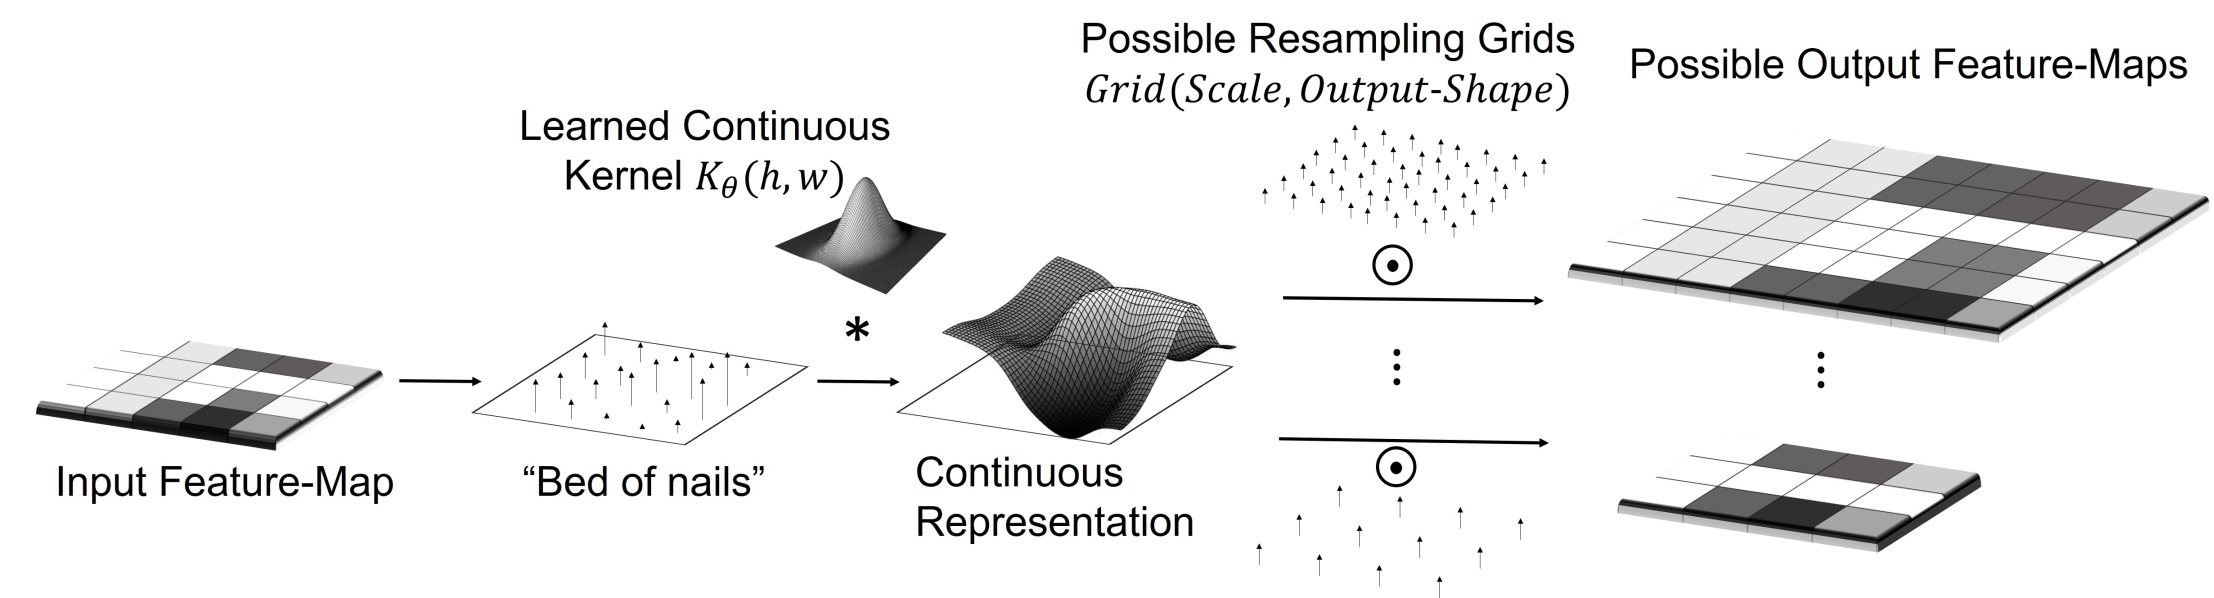
\includegraphics[width=1.05\textwidth]{figs/fig_underlying2.jpg}
    \caption{The underlying process of CC.
    % \niv{I guess "Grid" in 4th stage should be relabeled as "Resampling Grids" like referred in the text, or "Resampling beds of nails"? like in 2nd stage; it should be clear that stages 2,3,4 are all in the continuous domain, and stage 2 and 4 are simply the continuous representations of input/outpus images resp. so why not use the same terminology here?. In any case it should be consistent with the text, which it is not at the moment}
    }
    \label{fig:underlying}
\end{figure}



%%%%%%%%%%%%%%  Should  be moved to a later chapter: %%%%%%%%%%%%%%%
% \cite{azulay2018deep} Show that small translations to CNN inputs can drastically change the prediction. \cite{zhang2019shiftinvar} Further elaborates on lack of shift invariance due to aliasing and proposes improved antialiased netwrok components with low-pass-filters to ameliorate it.
%%%%%%%%%%%%%%%%%%%%%%%%%%%%%%%%%%%%%%%%%%%%%%%%%%%%%%%%%%%%%%%%%%%%%%%





% The basic building block of CNNs is the convolution (conv) layer. This is a layer that applies discrete convolution (actually, cross-correlation) to an input tensor, with a learned discrete filter. The filter is a set of weights that can be optimized during training and are fixed at inference. Most CNN models employ spatial resizing of feature-maps. Both upscaling and downscaling are common operations. Such resizing can either be a learned parametric operation or a fixed predetrmied one. Leraned downscaling is usually done by strided conv-layers. The stride is an integer size that can be seen as the inverse of the resizing factor. Learned upscaling can be done using transposed convolution. In both cases, there are many limitations: (i) The stride must be an integer. Consequently, a learned transformation that includes spatial resizing can only be done by an integer or inverse of an integer scale-factor. (ii) Once trained, the filter and stride are determined and cannot be dynamically modified at inference. (One can technically use a trained conv-layer with modified stride. This will be equivalent to subsmapling rather than principled resizing). (iii) Occurrence of artifacts, such as impaired shift-equivariance \cite{zhang2019shift, azulayweiss2019}. Transposed convolutions suffer from checkerboard artifact \cite{checkerboard}.



% There exist many untrainable resizing methods, mostly used for images, but usually differentiable and can be combined in a neural network. Usually they map output pixels to input locations and apply some fixed interpolation (nearest neighbor, linear, cubic etc.) on each channel separately. When the scale-factor is inverse of an integer, these methods can be formalized as a fixed strided convolution, since the interpolation weights are identical for all locations. Such resizing is principled; it follows a consistent rule across all scales and sub-pixel positions. These, however are not learned and do not operate any feature transform, only scaling.




% To execute the underlying process we must use discrete components
















% \subsection{Contributions}
% \begin{itemize}[noitemsep]
%   \setlength{\itemsep}{0pt}
%     \item We present a natural generalization of the 2d convolution layer, which considers sub-pixel locations consistently.
%     \item CC is the first learnable layer that can resize to any scale, including non-integer, upscaling, and different scale to each dimension.
%     \item  Unlike existing neural resizing layers (eg. Strided-conv, Pooling), CC is dynamic; the scale is determined at test-time, ant the operation is consistent across scales.
%     \item We show that common 2d conv-layers suffer from inherent misalignment that is ameliorated by CC.
%     \item CC enables gradual architectures that give rise to shift-invariance.
%     \item We present an adaptive Super-Resolution method to any scale determined at inference time.
%     \item We propose a superior method for blind Super-Resolution, by modeling the kernel as continuous and consistent throughout different scales.
    
% \end{itemize}



% 1. We present a natural generalization of the 2d convolution layer, which considers sub-pixel locations consistently.\\
% 2. CC is the first learnable layer that can resize to any scale. \\
% 3. Unlike existing neural resizing layers (eg. Strided-conv, Pooling), CC is dynamic; the scale is determined at test-time. \\
% 4. We show that common 2d conv-layers suffer from inherent misalignment that is ameliorated by CC.\\
% 5. CC enables gradual architectures that give rise to shift-invariance.\\
% 6. We present an adaptive Super-Resolution method to any scale determined at inference time.\\
% 7. We propose a superior method for blind Super-Resolution, by modeling the kernel as continuous and consistent throughout different scales.
